\chapter{Pendahuluan}

Bab Pendahuluan secara umum menceritakan landasan kerja dan arah kerja penulis tugas akhir, yang berfungsi untuk mengantar pembaca dalam memahami dan menganalisis laporan tugas akhir secara keseluruhan. Bab ini terdiri dari latar belakang, rumusan masalah, tujuan, batasan masalah, metodologi, dan jadwal pelaksanaan tugas akhir.

\section{Latar Belakang}
\label{sec:latarbelakang}

Teknologi dan internet adalah kebutuhan yang penting dalam kehidupan manusia di abad ke-21 ini. Salah satu bentuk teknologi modern paling berguna yang mudah diakses manusia adalah \emph{smartphone}, di mana akses internet sudah termasuk ke dalamnya. Berdasarkan penelitian yang dikumpulkan oleh \textcite{turner2022howmanysmartphones} pada bankmycell.com, pada tahun 2021 terdapat 6.37 miliar pengguna \emph{smartphone} di dunia atau sekitar 80.68\% dari populasi dunia, di antaranya 160.23 juta adalah penduduk Indonesia.

Banyak pekerjaan manusia yang dapat dilakukan dengan menggunakan berbagai jenis aplikasi yang dapat ditemukan dalam sebuah \emph{smartphone}. Menurut penelitian yang dilakukan oleh BusinessofApps, jumlah aplikasi pada iOS App Store ketika pertama kali diluncurkan pada tahun 2008 adalah 500, pada bulan November tahun 2021 angka tersebut melonjak menjadi 1.85 juta aplikasi. Pengguna Android memiliki lebih banyak pilihan dengan total 2.56 juta aplikasi di Google Play Store. Dengan banyaknya aplikasi tersebut, pada tahun 2020 pengguna \emph{smartphone} telah mengunduh aplikasi sebanyak 142.9 miliar kali, di antaranya 56.1 miliar unduhan adalah untuk aplikasi permainan \emph{mobile}.

Teknologi informasi yang semakin berkembang dapat meningkatkan kesejahteraaan digital, atau digital wellbeing, dari pengguna teknologi tersebut, beberapa caranya adalah meningkatkan koneksi sosial, mendukung kesehatan mental, dan mendukung kebiasaan sehat dengan fleksibilitas dalam praktik kerja. Namun teknologi informasi juga dapat menimbulkan akibat buruk yang memunculkan pola penggunaan teknologi yang tidak sehat. Beberapa contoh dampak buruk yang dimunculkan adalah mudahnya seseorang untuk kehilangan fokus, perasaan \emph{fear of missing out} (FoMO), serta kecanduan digital. Sifat-sifat buruk tersebut dapat lebih sering muncul ketika waktu yang dihabiskan pada dunia maya tidak diimbangi dengan waktu di dunia nyata. \parencite{ALMOURAD2021101778}

Pengaruh buruk seperti yang telah disebutkan di atas serta perilaku adiksi pada \textit{smartphone} telah memunculkan perhatian bagi peneliti di bidang \textit{Human Computer Interaction} (HCI) untuk melakukan studi terhadap kesengajaan untuk tidak menggunakan teknologi. Pada saat ini, terdapat banyak perangkat lunak pada \textit{smartphone} yang bertujuan untuk mengubah perilaku penggunanya, salah satunya dibuat oleh Google. \parencite{CHI2019SOCIALIZE} Untuk membantu penggunanya, Google memiliki aplikasi Digital Wellbeing agar pengguna dapat memanfaatkan teknologi untuk meningkatkan kualitas kehidupannya melainkan menjadi distraksi. Pada websitenya tentang Digital Wellbeing, \textcite{google2019digitalwellbeing} mengatakan: "We’re committed to giving everyone the tools they need to develop their own sense of digital wellbeing. So that life, not the technology in it, stays front and center." 


% Salah satu fitur yang terdapat pada aplikasi Digital Wellbeing adalah Focus Mode, sebuah fitur yang dapat membantu mengurangi distraksi dari \emph{smartphone} berbasis Android dengan cara memblokir sementara aplikasi yang dinilai sebagai distraksi. Focus Mode juga akan mendiamkan notifikasi yang masuk hingga waktu yang ditentukan. Waktu yang diterapkan untuk Focus Mode dapat diatur jadwalnya oleh pengguna. \parencite{android2019digitalwellbeing} Selama Focus Mode aktif, akan terdapat sebuah menu pada bagian notifikasi \emph{smartphone} dengan 2 buah fitur. Fitur "Take a break" yang berbentuk tombol ini dapat memberikan pengguna kembali akses untuk aplikasi yang diblok dengan pilihan waktu 5 menit, 15 menit, atau 30 menit. Tombol ini dapat digunakan jika pengguna ingin beristirahat dan menggunakan aplikasi yang diblok. Fitur "Turn off for now" yang juga berbentuk tombol dapat digunakan untuk memberhentikan Focus Mode hanya untuk hari tersebut. Tombol ini dapat digunakan jika pengguna merasa tugas yang perlu difokuskannya sudah selesai dan ingin menggunakan aplikasi yang diblok untuk sisa harinya. Masalah yang ditemukan dari Focus Mode terletak pada kedua fitur ini. Walau memerlukan interaksi lebih untuk "beristirahat", terdapat kemungkinan bagi pengguna untuk terus menerus mengakses aplikasi, dengan mengambil istirahat setiap beberapa menit sekali. Selain itu, fitur "Turn off for now" dapat disalahgunakan untuk menghindari Focus Mode secara keseluruhan.

\section{Rumusan Masalah}

Penggunaan tinggi \textit{smartphone} dapat mempengaruhi kesejahteraan digital dari penggunanya dalam cara yang negatif. Salah satu bentuk dari hubungan yang tidak baik antara \textit{smartphone} dan penggunanya adalah tingginya tingkat ketergantungan terhadap \textit{smartphone} hingga dapat mencapai tingkat adiksi. Penurunan kualitas hubungan tersebut dapat disebabkan oleh gangguan dari aplikasi pada \textit{smartphone} atau keinginan pengguna sendiri untuk menggunakannya. Dalam upaya memperbaiki hubungan tersebut, Google merilis aplikasi Digital Wellbeing yang bertugas untuk membantu pengguna \textit{smartphone} berbasis Android untuk mengatur kesehatan penggunaannya. Namun, dengan banyaknya aplikasi dengan tujuan serupa di \textit{marketplace} Google Play Store, dapat dilihat bahwa terdapat beberapa batasan pada aplikasi Digital Wellbeing. Maka dari itu, dapat disimpulkan rumusan masalah yang akan didalami dalam Tugas Akhir ini adalah sebagai berikut

\begin{enumerate}
  \item Apa \textit{usability goals} dan \textit{user experience goals} yang tepat untuk sebuah aplikasi pencegah distraksi?
  \item Bagaimana rancangan desain interaksi yang tepat untuk menyelesaikan masalah yang terdapat pada aplikasi pencegah distraksi Digital Wellbeing yang disusun menggunakan pendekatan \textit{user-centered design}?
  % \item Bagaimana rancangan desain interaksi yang tepat untuk menyelesaikan masalah yang terdapat pada aplikasi pencegah distraksi Digital Wellbeing?
  % \item Bagaimana prototipe aplikasi pencegah distraksi Digital Wellbeing dengan desain interaksi menggunakan pendekatan \emph{user-centered design}?
\end{enumerate}

\section{Tujuan}

Berdasarkan latar belakang dan rumusan masalah di atas, tujuan dari Tugas Akhir ini adalah untuk membuat sebuah prototipe aplikasi pencegah distraksi. Prototipe aplikasi tersebut memiliki desain interaksi yang dapat menyelesaikan masalah-masalah desain interaksi yang ditemukan pada alat Digital Wellbeing milik Google.


\section{Batasan Masalah}

Batasan masalah untuk implementasi solusi Tugas Akhir ini adalah sebagai berikut
\begin{enumerate}
  % \item Hasil akhir dari studi adalah solusi dalam bentuk prototipe aplikasi untuk \textit{smartphone} berbasis Android dengan versi OS lebih besar sama dengan versi Android 9.0.
  \item Responden penelitian adalah masyarakat Indonesia, dengan rentang umur 18 hingga 30 tahun.
  \item Hasil akhir dari studi adalah solusi dalam bentuk prototipe aplikasi yang didesain untuk \textit{smartphone} berbasis Android.
  % \item Pengujian akan dilakukan dengan membandingkan penggunaan \textit{smartphone} yang disertai bantuan aplikasi Digital Wellbeing dengan prototipe aplikasi solusi.
\end{enumerate}

\section{Metodologi}
\label{sec:metodologi}

Metodologi dalam perancangan solusi Tugas Akhir menggunakan pendekatan \textit{user-centered design} (UCD) yang mengikuti standar alur kerja dari ISO (\textit{International Organization for Standardization}) 9241-210:2010. Berikut adalah penjelasan dari setiap tahap UCD


\begin{figure}[h]
  \centering
  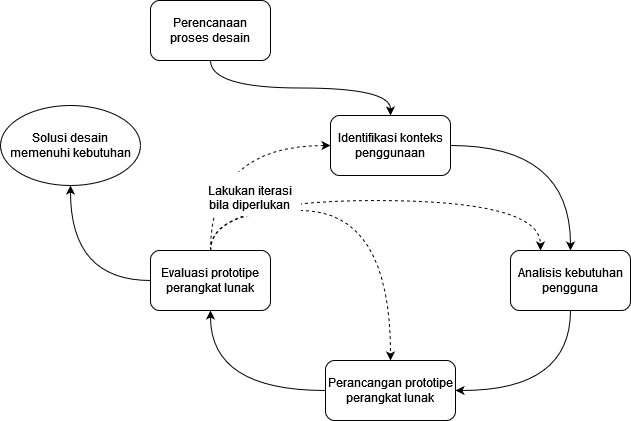
\includegraphics[width=0.9\textwidth]{chapter-1-method.png}
  \caption{Diagram alur pengerjaan \textit{User-Centered Design} (ISO 9241-210, 2010)}
  \label{fig:diagram_iso1}
\end{figure}

\begin{enumerate}
  \item Perencanaan proses desain
  \subitem Proses UCD diawali dengan tahap persiapan, yaitu proses perancangan terhadap lingkup aplikasi yang dibuat serta perencanaan untuk pengambilan data. Lingkup dari aplikasi termasuk jenis antarmuka dan \textit{platform} yang dipilih untuk implementasi, lingkup fungsionalitas aplikasi, serta target pengguna aplikasi. Sedangkan perencanaan pengambilan data dilakukan dengan cara analisis ulasan aplikasi dan wawancara pengguna.

  \item Identifikasi konteks penggunaan
  \subitem Pada tahap ini dilakukan pengumpulan data pengguna melalui analisis ulasan pengguna dan wawancara sesuai dengan kebutuhan. Data yang didapatkan akan dianalisis untuk mengungkapkan perilaku dan permasalahan pengguna tentang aplikasi. Fungsionalitas dari aplikasi juga penting untuk mengerti konteks penggunaannya. Berdasarkan data riset tersebut akan dibentuk persona pengguna, yang kemudian akan dianalisis untuk mendapatkan kebutuhan, tujuan dan kegiatan pengguna, serta skenario pengguna.
   
  \item Penentuan kebutuhan perangkat lunak
  \subitem Tahap ini terdiri dari analisis tipe interaksi, analisis fitur, analisis prinsip desain, serta \textit{user experience goals} dan \textit{usability goals}. Fitur-fitur yang terkumpul akan menjadi bahan implementasi pada tahap selanjutnya.
  
  \item Perancangan prototipe perangkat lunak
  \subitem Rancangan kebutuhan pengguna yang sudah dikumpulkan pada tahap sebelumnya akan kemudian diimplementasikan, mulai dari \textit{low-fidelity prototype}, dilanjut dengan \textit{high-fidelity prototype} berupa prototipe aplikasi. Proses ini dilakukan secara iteratif bersamaan dengan tahap evaluasi.
  
  \item Evaluasi prototipe perangkat lunak
  \subitem Tahap evaluasi dilakukan untuk menguji kemampuan solusi desain yang telah dirancang dalam memenuhi kebutuhan pengguna dan \textit{user experience goals} serta \textit{usability goals} yang ditargetkan. Hasil evaluasi akan menentukan apakah desain yang diuji perlu diperbaiki dalam proses iterasi.
  
\end{enumerate}


\section{Sistematika Pembahasan}

Subbab ini berisi penjelasan ringkas isi per bab. Penjelasan ditulis satu paragraf per bab buku.
